\documentclass{cubeamer}

\title{Título da Apresentação}
\subtitle{Nome do Evento}
\author[João Vítor Silva Mendes]{João Vítor Silva Mendes}
\date{\today} % or whatever the date you are presenting in is
\institute[SENAI CIMATEC]{SENAI CIMATEC -  STUDENT BRANCH CHAPTER - ROBOTICS AND AUTOMATION SOCIETY}
% \copyrightnotice{Published by the American Institute of Aeronautics and Astronautics, Inc., with permission}

\begin{document}

\maketitle

\cutoc

\section{Introduction}

\begin{frame}{Frame Title}
    \begin{itemize}
        \item Use
        \item Figures,
        \item Do
        \item Not
        \item Use
        \item Bullet
        \item Points
    \end{itemize}
\end{frame}

\begin{frame}{Use meaningful titles that actually provide information}
    \begin{columns}
        \begin{column}{0.6\textwidth}
            \begin{figure}
                \centering
                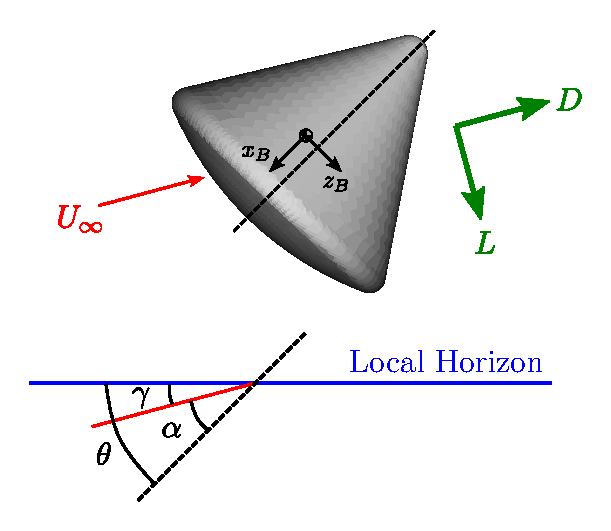
\includegraphics[height = 0.7\textheight]{img/example.pdf}
                \caption{Fancy Thing from \textit{Source et al.}}
            \end{figure}
        \end{column}
        \begin{column}{0.4\textwidth}
            \begin{itemize}
                \item Some
                \item Interesting
                \item Points
            \end{itemize}
        \end{column}
    \end{columns}
\end{frame}

\section{A Section}

\begin{frame}{Make your presentation interactive}
    \begin{cublock}[What about a question to the audience?]
        \begin{overlayarea}{\textwidth}{\baselineskip}
            \only<2->{Followed by the answer.}
        \end{overlayarea}
    \end{cublock}
\end{frame}

% Q&A
\begin{frame}[standout]
    \Huge\textsc{Thank You}
    
    \vfill
    
    \LARGE\textsc{Questions?}
\end{frame}

\appendix

\begin{frame}{Backup slides go here}
    
\end{frame}

\end{document}
